\documentclass[preprint,12pt,ntfdMod]{elsarticle}
\usepackage{graphicx}
\usepackage{color}
\usepackage[numbered,bw]{mcode}
\usepackage{amsmath}
\usepackage{amsfonts}
\usepackage{hyperref}
\usepackage{esint}
\usepackage{units}
\usepackage[protrusion=true,expansion]{microtype}
\hypersetup{
	bookmarks=true,         % show bookmarks bar?
	unicode=false,          % non-Latin characters in Acrobat’s bookmarks
	pdftoolbar=true,        % show Acrobat’s toolbar?
	pdfmenubar=true,        % show Acrobat’s menu?
	pdffitwindow=false,     % window fit to page when opened
	pdfstartview={FitH},    % fits the width of the page to the window
	pdftitle={My title},    % title
	pdfauthor={Author},     % author
	pdfsubject={Subject},   % subject of the document
	pdfcreator={Creator},   % creator of the document
	pdfproducer={Producer}, % producer of the document
	pdfkeywords={keyword1} {key2} {key3}, % list of keywords
	pdfnewwindow=true,      % links in new window
	colorlinks=true,       % false: boxed links; true: colored links
	linkcolor=red,          % color of internal links
	citecolor=green,        % color of links to bibliography
	filecolor=magenta,      % color of file links
	urlcolor=cyan           % color of external links
}
\usepackage{verbatim}
\usepackage{relsize}
\usepackage{lipsum}
\usepackage{caption}
\captionsetup[figure]{name=Fig.,labelfont=bf}
\usepackage{tocloft}
\setlength{\cftbeforesecskip}{2pt}

\definecolor{lightgray}{gray}{0.5}
\setlength{\parindent}{0pt}

%c from texinfo.tex
\def\ifmonospace{\ifdim\fontdimen3\font=0pt }
%c C plus plus
\def\C++{%
\ifmonospace%
    C++%
	\else%
	    C\kern-.1667em\raise.30ex\hbox{\smaller{++}}%
		\fi%
		\spacefactor1000 }
\lstset{%
xleftmargin=8mm,%
xrightmargin=8mm,%
framexleftmargin=6mm,%
xleftmargin=6mm,%
breaklines=true}

\author[rss]{Felix Dietzsch}
\address[rss]{Institut für Chemieingenieurwesen und Energieverahrenstechnik,...}
\title{Small post processor}
\begin{document}
\maketitle 
\tableofcontents

    
    
\section{Contents}

\begin{itemize}
\setlength{\itemsep}{-1ex}
   \item Clear complete workspace
   \item Read data files
   \item Set neccessary parameters
   \item Compute 3D spectrum
   \item Compute dissipation and turbulent kinetic energy
   \item Kolmogrov properties
   \item Compute model spectra
   \item Compute correlations
\end{itemize}


\section{Clear complete workspace}

\begin{par}
For new Matlab projects best practise is to clear the complete workspace and the command window. It is also a good habit to close all remaining figures since Matlab does not automatically open a new window each time a plot call is invoked.
\end{par} \vspace{1em}
\begin{lstlisting}
path('./functions',path) % add functions directory the Matlab path
close all % close all figures
clear all % clear workspace
clc % clear command window
set(0,'DefaultFigureWindowStyle','docked')
[datadir,flag]=ClearWs();
\end{lstlisting}
\begin{par}

The above mentioned clears are performed in the function \verb|ClearWs|.
In addition some basic parameters like the name of the data
directory or the dimensionality of the problem are also defined.
\lstinputlisting{../functions/ClearWs.m}

\end{par} \vspace{1em}


\section{Read data files}

\begin{par}

During the evaluation of the function \verb|ReadData| all data files
neseccary for the calculation of the spectrum and the correlation
coefficients are read, namely the velocity components. In addition the
import operations are enclosed in a \lstinline!tic;!$\ldots$
\lstinline!;toc! block
measuring the time needed for reading the ASCII data. What you should
get from the tic/toc
block is that most of the time is spend during data I/O
(Input/Output operations), nearly \unit[220]{s}. The actual computation
needs only about \unit[8]{s}. What you can easily calculate from this is
that the
computation of the spectrum is nearly 27 times faster then the data
import. Why the computation of Fourier transforms is that fast we will
come to that later.
Although the ASCII
data format ist not the prefered choice in terms of speed and size, we
will use it since other
methodologies require additional knowledge of data processing. Just for
your information a very famous and highly protable data format is
\href{http://www.hdfgroup.org/HDF5/}{hdf5}. It is a software library that
runs on a range of computational platforms, from laptops to massively
parallel systems and implements a high-level API (Application
programming interface) with C, \C++, Fortran 90,
and Java interfaces. Besides its hierarchical
structure it is highly optimized for parallel I/O operations and can be
read by nearly all data processing tools.

\end{par} \vspace{1em}
\begin{par}
[uvel,vvel,wvel,time\_read] = ReadData(datadir,flag,'uvel','vvel','wvel');
\end{par} \vspace{1em}
\begin{lstlisting}
test=importdata('data/3D/CFX_velocity_field.dat');
uvel=reshape(test(:,1),33,33,33);
vvel=reshape(test(:,2),33,33,33);
wvel=reshape(test(:,3),33,33,33);
\end{lstlisting}
\begin{par}

\lstinputlisting{../functions/ReadData.m}

\end{par} \vspace{1em}


\section{Set neccessary parameters}

\begin{par}

For further computations it is important to define some parmeters of the
DNS simulation such as
\begin{itemize}
  \item Number of grid points in on direction $n_{p}$,
  \item Physical length of one direction $L_x$,
  \item Physical grid spacing $\triangle x$,
  \item Kinematic viscosity $\nu$.
\end{itemize}

\end{par} \vspace{1em}
\begin{lstlisting}
[u,v,w,dim,Lx,dx,nu]=Params(uvel,vvel,wvel);
% u=u-mean2(u);
% v=v-mean2(v);
% w=w-mean2(w);
\end{lstlisting}
\begin{par}

\lstinputlisting{../functions/Params.m}

\end{par} \vspace{1em}


\section{Compute 3D spectrum}

\begin{par}

The core of the code is contained in the function
\lstinline!PowerSpec!. It computes the three dimensional energy spectrum
from the given velocity fields, obtained from a direct numerical
simulation. Although the theoretical analysis is
relatively demanding compared to one dimensional spectra its worth
investing the effort. The theory of one dimensional spectra relies
on the assumption that the propagation of spectral waves ($\kappa_1$)
is in the
direction of the observed velocity fields or to say it differently one
dimenional spectra and correlation functions are Fourier transform pairs.
The theory of correlation functions will be discussed in a later section.
A key drawback of this theory is that the calculated spectrum has
contributions from all wavenumbers $\boldsymbol\kappa$, so that the
magnitude of $\boldsymbol\kappa$ can be appreciably larger than
$\kappa_1$. This phenomenon is called aliasing.\\
In order to avoid aliasing effects usually connected with a one
dimensional spectrum it is also possible to produce correlations that
involve all possible directions. The three dimensional Fourier
transformation of such a correlation produces a spectrum that not only
depends on a single wavenumber but on the wavenumber vector $\kappa_i$.
Though the directional information contained in $\kappa_i$ eliminates the
aliasing problem the complexity makes a physical reasoning impossible.
For homogeneous isotropic turbulence the situation can be simplified by
integrating the three dimensional spectrum over spherical shells. The
idea of this integration is illustrated in Fig. \ref{fig:shell_int}
\begin{figure}
  \centering
  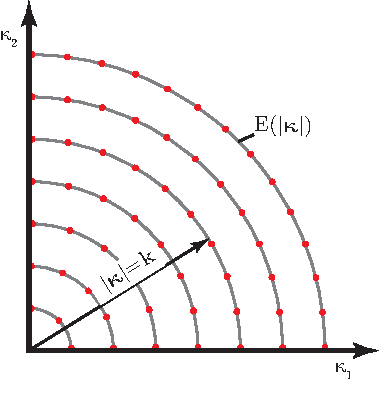
\includegraphics[scale=1]{shell_integration}
  \caption{Illustration of the two dimensional shell integration}
  \label{fig:shell_int}
\end{figure}

\end{par} \vspace{1em}
\begin{par}

  \begin{equation}
      E(\kappa) = \oiint E(\boldsymbol\kappa)\mathrm{d}S(\kappa)
                = \oiint \frac{1}{2}\,\Phi_{ii}(\boldsymbol\kappa)\mathrm{d}S(\kappa)
  \end{equation}
  Since the surface of a sphereis completly determined by its radius the
  surface integral can be solved analytically.
  \begin{equation}
      \oiint(\,)\mathrm{d}S(\kappa) = 4\pi\kappa^2\cdot(\,)
  \end{equation}
This leads to
  \begin{equation}
      E(|\kappa|) = \frac{1}{2}\,\Phi_{ii}(|\boldsymbol\kappa|)
  \end{equation}

\end{par} \vspace{1em}
\begin{lstlisting}
[spectrum,k,time_spec] = PowerSpec(u,v,w,Lx,dim);
\end{lstlisting}
\begin{par}

\lstinputlisting{../functions/PowerSpec.m}

\end{par} \vspace{1em}


\section{Compute dissipation and turbulent kinetic energy}

\begin{par}

  The function \lstinline!SpecProp! calculates the kinetic energy both
  from the velocities and the previously computed spectrum. The latter
  one is calcualted by
  \begin{equation}
      k = \int E(\kappa)\,\mathrm{d}\kappa\qquad \kappa=|\boldsymbol\kappa|
  \end{equation}
  A second integral, also evaluated in this routine, gives the value
  of the Dissipation
  \begin{equation}
      \epsilon = 2\int\nu\kappa^2 E(\kappa)\,\mathrm{d}\kappa
  \end{equation}

\end{par} \vspace{1em}
\begin{lstlisting}
[Dissipation,kin_E_Sp,kin_E_Ph,up] = SpecProp(spectrum,k,nu,u,v,w,dim);
kin_E_Ph
kin_E_Sp
\end{lstlisting}
\begin{par}

\lstinputlisting{../functions/SpecProp.m}

\end{par} \vspace{1em}


\section{Kolmogrov properties}

\begin{lstlisting}
[eta,u_eta,tau]=KolmoScale(nu,Dissipation);
eta
u_eta
tau
\end{lstlisting}
\begin{par}

The content of \verb|KolmoScale| reads
\lstinputlisting{../functions/KolmoScale.m}

\end{par} \vspace{1em}


\section{Compute model spectra}

\begin{lstlisting}
PlotModelSpec(k,spectrum,Dissipation,up,Lx,eta,nu);
\end{lstlisting}
\begin{par}

The content of \verb|PlotModelSpec| reads
\lstinputlisting{../functions/PlotModelSpec.m}

\end{par} \vspace{1em}


\section{Compute correlations}

\begin{par}
Computing a correlation can be a tedious work (requireing tremendeous effort) especially if you have large data sets. From theory it is well known that the multiplication of the transform of a data set and its complex conjugate are an accurate representation of the correlation function. Using the FFT approach this gives an enormeous speed advantage. Since we already computed the veloity correlation tensor we may use this result in order to compute the correlation tensor.
\end{par} \vspace{1em}
\begin{par}

  \begin{equation}
      R_{ij} = \frac{cov(U_i,U_j)}{\sqrt{\sigma_i^2\,\sigma_j^2}}
             = \frac{\left<u_i'\,u_j'\right>}{\sqrt{\sigma_i^2\,\sigma_j^2}}
  \end{equation}

\end{par} \vspace{1em}
\begin{lstlisting}
[R11,R22,r,R1,R2,R3]=Correlation(u,v,w,Lx,dim);
close all
figure
plot(r,R11,r,R22)
legend('R11','R22')
\end{lstlisting}
\begin{par}

The content of \verb|Correlation| reads
\lstinputlisting{../functions/Correlation.m}

\end{par} \vspace{1em}
\begin{lstlisting}
close all
sohm=importdata('data/3D/SPECTRUM_00.SET');
h=loglog(sohm(:,1),sohm(:,2),'*-b');hold on
set(h,'LineWidth',1);
h=loglog(k,spectrum,'r-s');
set(h,'LineWidth',1);
legend('Sohm','Dietzsch')
saveas(gcf,'spectrum.eps','psc2')
\end{lstlisting}



\end{document}
    
